\newpage
\section{METHODOLOGY}

The literature review has exposed us to a variety of ways (some simple, some complex) used in the problem domain. In fact, no two papers had remotely similar
methodologies; they varied in at least one of feature extraction, classification algorithm used or the Genre themselves.
The features selected are mostly based on the results obtained in \cite{LiTao2003} where FFT, MFCC, Pitch and Beat were investigated and a
combination of all those features were found to give the best results. 
Although SVM, K-NN, Variants of Neural Networks, were found to be the most commonly used algorithms. However, as we had decided to try out one unsupervised
method and one supervised method, we were mostly interested in how K-means and ANN were used.
\par Also we were focusing on K-means for this mid-term, so we looked at the two papers \cite{Haggblade2011}, \cite{Tzanetakis1992} that had made use of it. We also
went over lots of other papers \cite{Apon2006}, \cite{Jain2010}, \cite{Hamerly2002} related to the algorithm itself (not directly related to Music Classification). How
the literature affected our methodology will be discussed in the sections pertaining to the methodologies used.  

\subsection{System Block Diagram}
The main components of our system are:
\begin{itemize}
        \item\textbf{Audio Sampling - }It makes use of MP3 decoder and OGG decoder to sample the audio.  
        \item\textbf{Feature Extraction - }The relevant features are extracted in this stage.
        \item\textbf{Feature Integration - }The extracted features are integrated into a single JSON file.
        \item\textbf{Learning Algorithm - }The learning algorithm uses the feature file to create a model for classification.
        \item\textbf{Validation - }The last stage involves validating the results obtained.
\end{itemize}
\newpage
The block diagram is as follows:

\begin{figure}[h!]
        \centering
        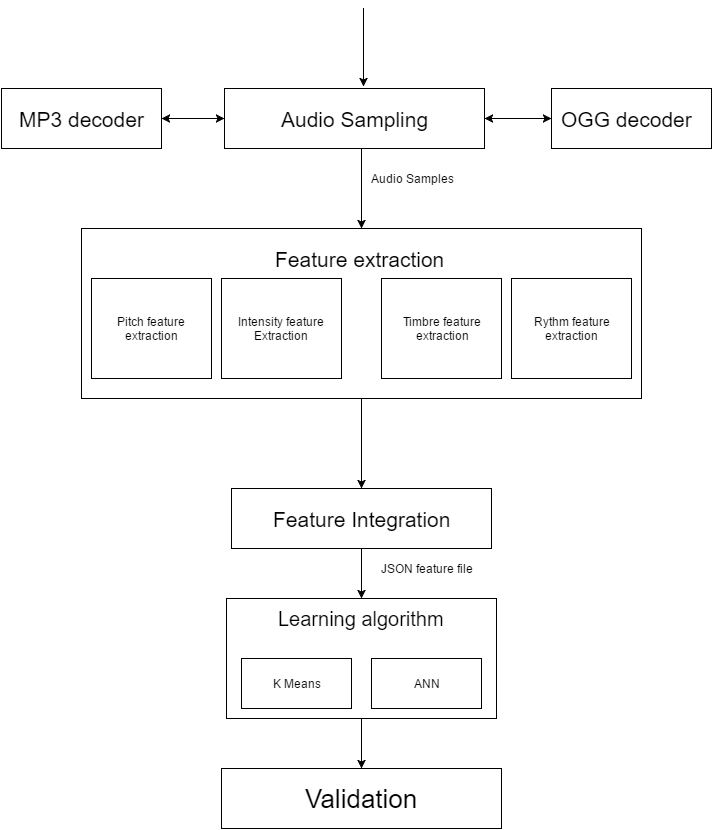
\includegraphics[width=120mm]{resources/system.jpg}
        \caption{System Block Diagram}
        \label{fig:figure2}
\end{figure}

\subsection{Data Collection}
As we have chosen five genres for our classification ourselves, we decided to first collect data based on our own view. For that we will be using our
own music collection and collect remaining from our friend.Then according to the result we will be opting for the standard database of music provided
by sites like marsyas,etc.

\subsection{Feature Extraction}

\subsubsection{Overview}
Feature extraction is the process of computing a compact numerical representation that can be used to characterize a segment of audio. It is observed
that the feature selection always plays an important role in building a good pattern classifier. Once the features are extracted standard machine learning
techniques which are independent of the specific application area can be used. 
\par  After considering many commonly used features, we decided on using the intensity, rhythm, timbral and pitch as the key features for our initial
classification task. 
\par For this mid-term, we have completed the extraction of the first three of the four features: intensity, rhythm and timbre (as MFCC). 

\subsubsection{Overview of JAVA sampled package and AudioSystem class}

The javax.sound.sampled package is fundamentally concerned with audio transport — in other words, the Java Sound API focuses on playback and capture. The
central task that the Java Sound API addresses is how to move bytes of formatted audio data into and out of the system. 

To make use of the Java Sound API, at least three things are necessary: formatted audio data, a mixer, and a line. The following provides an overview of
these concepts.

\begin{enumerate}[a.] 
        \item \textbf{Data Formats -} 
                A data format provides information on how to interpret a series of bytes of "raw" sampled audio data, such as samples that have already
                been read from a sound file, or samples that have been captured from the microphone input. It has various use cases, for example, how many
                bits constitute one sample (the representation of the shortest instant of sound), and the sound's sample rate (how fast the samples are supposed to
                follow one another). In the Java Sound API, a data format is represented by an AudioFormat object, which includes the following attributes:
                \begin{itemize}
                        \item Encoding technique, usually pulse code modulation (PCM)
                        \item Number of channels (one for mono, two for stereo, etc.)
                        \item Sample rate (number of samples per second, per channel)
                        \item Number of bits per sample (per channel)
                        \item Frame rate
                        \item Frame size in bytes
                        \item Byte order (big-endian or little-endian)
                \end{itemize}

                \par PCM is one kind of encoding of the sound waveform. The Java Sound API includes two PCM encodings that use linear quantization of amplitude,
                and signed or unsigned integer values. Linear quantization means that the number stored in each sample is directly proportional (except for any
                distortion) to the original sound pressure at that instant—and similarly proportional to the displacement of a loudspeaker or eardrum that is
                vibrating with the sound at that instant. 
                \par A frame contains the data for all channels at a particular time. For PCM-encoded data, the frame is simply the set of simultaneous
                samples in all channels, for a given instant in time, without any additional information. In this case, the frame rate is equal to the
                sample rate, and the frame size in bytes is the number of channels multiplied by the sample size in bits, divided by the number of bits
                in a byte. For other kinds of encodings, a frame might contain additional information besides the samples, and the frame rate might be
                completely different from the sample rate. For the MP3 (MPEG-1 Audio Layer 3) encoding, which is not explicitly mentioned in the current
                version of the Java Sound API, but which could be supported by an implementation of the Java Sound API or by a third-party service provider. In
                MP3, each frame contains a bundle of compressed data for a series of samples, not just one sample per channel. Because each frame encapsulates
                a whole series of samples, the frame rate is slower than the sample rate. The frame also contains a header. Despite the header, the frame size
                in bytes is less than the size in bytes of the equivalent number of PCM frames. (After all, the purpose of MP3 is to be more compact than PCM
                data.) For such an encoding, the sample rate and sample size refer to the PCM data that the encoded sound will eventually be converted into
                before being delivered to a digital-to-analog converter (DAC).

        \item \textbf{File Formats -} 
                A file format specifies the structure of a sound file, including not only the format of the raw audio data in the file, but also other information
                that can be stored in the file. 

                \begin{itemize}
                        \item In the Java Sound API, a file format is represented by an AudioFileFormat object, which contains:
                        \item The file type (WAVE, AIFF, etc.)
                        \item The file's length in bytes
                        \item The length, in frames, of the audio data contained in the file
                        \item An AudioFormat object that specifies the data format of the audio data contained in the file
                \end{itemize}

        \item \textbf{Mixer -} 
                Many application programming interfaces (APIs) for sound make use of the notion of an audio device. A device is often a software interface
                to a physical input/output device. For example, a sound-input device might represent the input capabilities of a sound card, including a
                microphone input, a line-level analog input, and perhaps a digital audio input. In the Java Sound API, devices are represented by Mixer
                 objects. The purpose of a mixer is to handle one or more streams of audio input and one or more streams of audio output. In the typical
                case, it actually mixes together multiple incoming streams into one outgoing stream. A Mixer object can represent the sound-mixing capabilities
                of a physical device such as a sound card, which might need to mix the sound coming in to the computer from various inputs, or the sound coming
                from application programs and going to outputs.

        \item \textbf{Line -} 
                A line is an element of the digital audio "pipeline" that is, a path for moving audio into or out of the system. Usually the line is a path into or out of a mixer
                (although technically the mixer itself is also a kind of line). 

\end{enumerate}

\textit{Accessing Audio System Resources}

The Java Sound API takes a flexible approach to system configuration. Different sorts of audio devices (mixers) can be installed on a computer. The
API makes few assumptions about what devices have been installed and what their capabilities are. Instead, it provides ways for the system to report
about the available audio components, and ways for the program to access them.

\textit{The AudioSystem Class}

The AudioSystem class acts as a clearinghouse for audio components, including built-in services and separately installed services from third-party
providers. AudioSystem serves as an application program's entry point for accessing these installed sampled-audio resources. AudioSystem can be queried
to learn what sorts of resources have been installed, and then obtain access to them. For example, an application program might start out by asking the
 AudioSystem class whether there is a mixer that has a certain configuration, such as one of the input or output configurations illustrated earlier in
the discussion of lines. From the mixer, the program would then obtain data lines, and so on.

Here are some of the resources an application program can obtain from the AudioSystem:

\begin{itemize}
        \item \textbf{Mixers -} A system typically has multiple mixers installed. There is usually at least one for audio input and one for audio output. There
                might also be mixers that don't have I/O ports but instead accept audio from an application program and deliver the mixed audio back to the program. The
                 AudioSystem class provides a list of all of the installed mixers.
        \item \textbf{Lines -} Even though every line is associated with a mixer, an application program can get a line directly from the AudioSystem,
                without dealing explicitly with mixers.
        \item \textbf{Format conversions -} An application program can use format conversions to translate audio data from one format to another.
        \item \textbf{Files and streams -} The AudioSystem class provides methods for translating between audio files and audio streams. It can
                also report the file format of a sound file and can write files in different formats.
\end{itemize}


\subsubsection{Audio Sampling}
Although Audio sampling is not part of the actual feature extraction process, it does form the basis for further processing. It involves the
reduction of a continuous audio signal to a discrete audio signal. To sample the audio signal we have used the java sound api for .wav file
and mp3spi library for .mp3 files.
\begin{figure}[h]
        \centering
        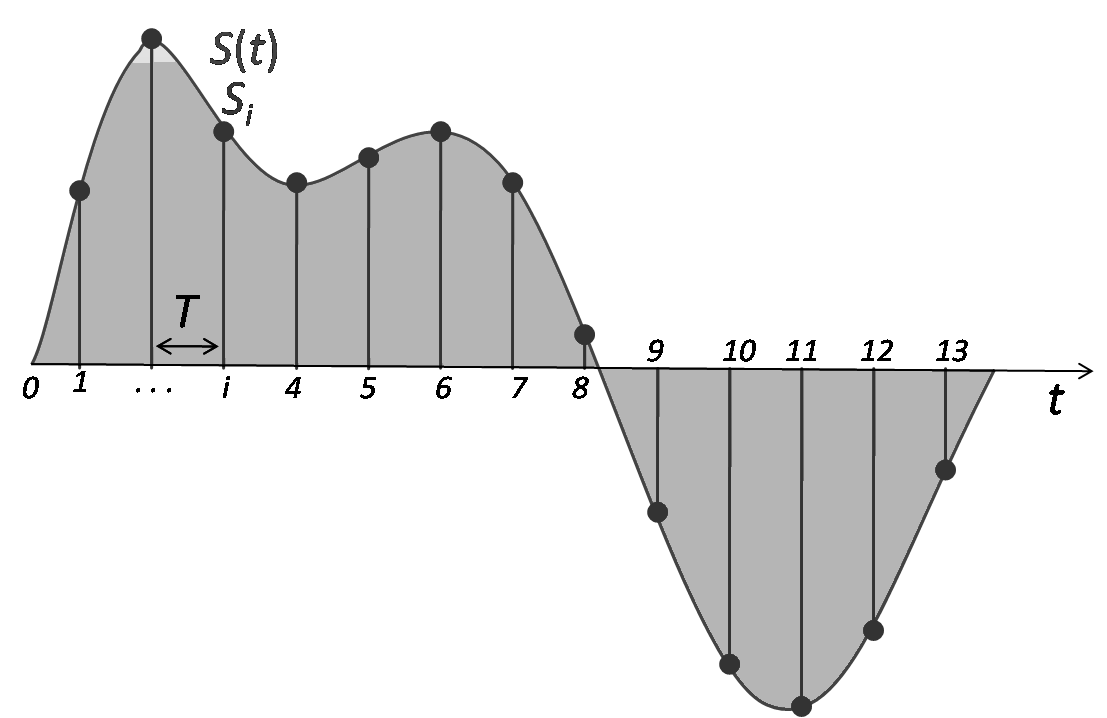
\includegraphics[width=100mm]{resources/audiosample.png}
        \caption{Sampling of an audio signal}
        \label{fig:figure3}
\end{figure}

\subsubsection{Timbral Features}
The main point to understand about speech is that the sounds generated by a human are filtered by the shape of the vocal tract including tongue, teeth etc. This shape
determines what sound comes out. If we can determine the shape accurately, this should give us an accurate representation of the phoneme being produced. The shape of
the vocal tract manifests itself in the envelope of the short time power spectrum, and the job of MFCCs is to accurately represent this envelope.
\par Many existing researchers have shown that mel-frequency cepstral coefficients (MFCCs), so called spectral shapes and spectral contrast are
the best features for analyzing the music. The mel-frequency cepstrum (MFC) is a representation of the short-term power spectrum of a sound, based
on a linear cosine transform of a log power spectrum on a nonlinear mel scale of frequency. Mel-frequency cepstral coefficients (MFCCs) are coefficients
that collectively make up an MFCC. They are derived from a type of cepstral representation of the audio clip (a nonlinear ”spectrum-of-a-spectrum”).\\
\textbf{MFCC Algorithm}

\begin{figure}[h]
        \centering
        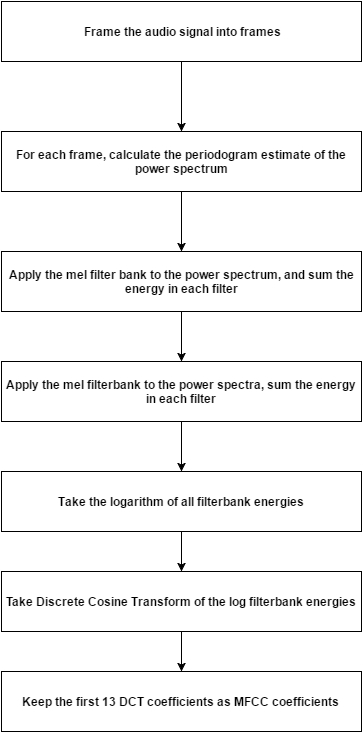
\includegraphics{resources/mfcc.jpg}
        \caption{MFCC component}
        \label{fig:figure4}
\end{figure}
We start with a speech signal, which we sample at 44100Hz.
\begin{enumerate}[1)]
        \item Frame the signal into 20-40 ms frames. 25ms is standard. This means the frame length for a 16kHz signal is 0.025*16000 = 400 samples. Frame step
                is usually something like 10ms (160 samples), which allows some overlap to the frames. The first 400 sample frame starts at sample zero, the
                next 400 sample frame starts at sample 160 etc. until the end of the speech file is reached. If the speech file does not divide into an even
                number of frames, pad it with zeros so that it does.
                \par The next steps are applied to every single frame, one set of 12 MFCC coefficients is extracted for each frame. A short aside on notation: we
                call our time domain signal S(n). Once it is framed we have where $S_i(n)$ ranges over 1-400 (if our frames are 400 samples) and i ranges over
                the number of frames. When we calculate the complex DFT, we get $S_i(k)$ where the i denotes the frame number corresponding to the time-domain frame and $P_i(s)$ then the power spectrum of frame i. 
        \item  To take the Discrete Fourier Transform of the frame, perform the following:
                \begin{equation}
                        S_i(k) = \sum_{n=1}^{N}(S_i(n)h(n)\mathrm{e}^{2\pi kn/n})    \hspace{20mm}for 1<k<K 
                \end{equation}
                where h(n) is an N sample long analysis window  (e.g. hamming window), and K is the length of the DFT.
                The periodogram-based power spectral estimate for the speech is $S_i(n)$ is given by: 
                \begin{equation}
                        P_i(k)=\frac{1}{N} |S_i(k)^2|
                \end{equation}
                This is called the Periodogram estimate of the power spectrum. We take the absolute value of the complex fourier transform, and square the result.
                We would generally perform a 512 point FFT and keep only the first 257 coefficents.
        \item  Compute the Mel-spaced filterbank. This is a set of 20-40 (26 is standard) triangular filters that we apply to the
                periodogram power spectral estimate from step two. Our filterbank comes in the form of 26 vectors of length 257
                (assuming the FFT settings from step two. Each vector is mostly zeros, but is non-zero for a certain section of the
                spectrum. To calculate filterbank energies we multiply each filterbank with the power spectrum, then add up the
                coefficents. Once this is performed we are left with 26 numbers that give us an indication of how much energy was
                in each filterbank. For a detailed explanation of how to calculate the filterbanks see below. Here is a plot to
                hopefully clear things up:
                \begin{figure}[h]
                        \centering
                        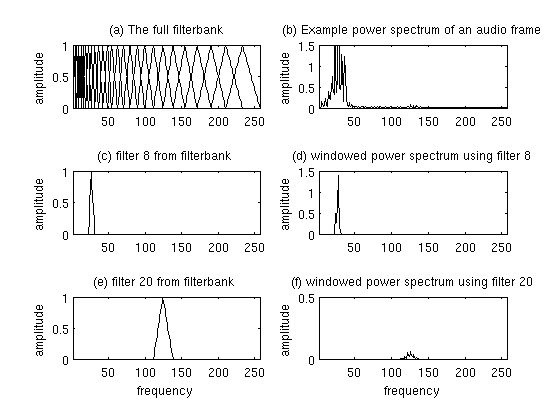
\includegraphics{resources/mfcc.png}
                        \caption{MFCC Calculation spectrum}
                        \label{fig:figure5}
                \end{figure}
        \item Take the log of each of the 26 energies from step three. This leaves us with 26 log filterbank energies. 
        \item Take the Discrete Cosine Transform (DCT) of the 26 log filterbank energies to give 26 cepstral coefficents. For
                ASR, only the lower 12-13 of the 26 coefficients are kept.
\end{enumerate}

The resulting features (12 numbers for each frame) are called Mel Frequency Cepstral Coefficients.

\subsubsection{Rhythmic Features}
Rhythmic features characterize the movement of music signals over time and contain information such as the regularity of the rhythm, beat tempo, and time signature. The
feature set for representing rhythm structure is usually extracted from the beat histogram. Tzanetakis \cite{Tzanetakis2002} used a beat histogram built from the autocorrelation
function of a signal to extract rhythmic features.
\par Simulating a physical phenomena which obeys to known mathematical equations is, with a number of approximations, always feasible. But what about
more abstract concepts, such as feelings, which do not follow any laws? The simplest things we can feel are often the hardest things to capture in a
program. Beat detection follows this rule : feeling the beat of a song comes naturally to humans or animals. Indeed it is only a feeling one gets when
listening to a melody, a feeling which will make you dance in rhythm or hit a table with your hands on the melody beats. 
\par The human listening system determines the rhythm of music by detecting a pseudo – periodical succession of beats. The
signal which is intercepted by the ear contains a certain energy, this energy is converted into an electrical signal which the brain interprets.
Obviously, The more energy the sound transports, the louder the sound will seem. But a sound will be heard as a beat only if his energy is largely
superior to the sound's energy history, that is to say if the brain detects a brutal variation in sound energy. Therefore if the ear intercepts a
monotonous sound with sometimes big energy peaks it will detect beats, however, if you play a continuous loud sound you will not perceive any
beats. Thus, the beats are big variations of sound energy.
\par To detect the beats we have used the Frequency selected sound energy algorithm.\\
Every 1024 samples:
\begin{enumerate}
        \item Compute the FFT on the 1024 new samples taken in ($a_n$) and ($b_n$). The FFT inputs a complex numeric signal. We will say ($a_n$) is the
                real part of the signal and ($b_n$) the imagenary part. Thus the FFT will be made on the 1024 complex values of: 
                \begin{equation}
                        a_n + i(b_n)
                \end{equation}
        \item From the FFT we obtain 1024 complex numbers. We compute the square of their module and store it into a new 1024 buffer. This buffer (B) contains
                the 1024 frequency amplitudes of our signal.
        \item Divide the buffer into 32 subbands, compute the energy on each of these subbands and store it at ($E_s$). Thus ($E_s$) will be 32 sized
                and $E_s[i]$ will contain the energy of subband 'i': 
                \begin{equation}
                        E_s[i]=\frac{32}{1024}*\sum_{k=i*32}^{(i+1)*32}{B[k]}
                \end{equation}
        \item Now, to each subband 'i' corresponds an energy history buffer called ($E_i$). This buffer contains the last 43 energy computations for
                the 'i' subband. We compute the average energy $<E_i>$ for the 'i' subband simply by using:   
                \begin{equation}
                        E_i[0]=\frac{1}{43}\times\sum_{k=0}^{42}{E_i[k]}
                \end{equation}
        \item Shift the sound energy history buffers ($E_i$) of 1 index to the right. We make room for the new energy value of the subband 'i' and flush the oldest.
        \item Pile in the new energy value of subband 'i' : $E_s[i]$ at $E_i[0]$.   
                \begin{equation}
                        E_i[0]=E_s[i]
                \end{equation}
        \item For each subband 'i' if $E_s[i]>(C*E_i)$ we have a beat.
\end{enumerate}

\subsubsection{Intensity Features}
Sound intensity also known as acoustic intensity is defined as the sound power per unit area. The usual context is the noise measurement of sound intensity
in the air at a listener’s location11 as a sound energy quantity. Intensity is approximated by the signals root mean square (RMS). The true RMS value of the
input signal is calculated over a running average window of one cycle of the specified fundamental frequency.
Procedure taken: 
\begin{enumerate}
        \item Input the WAV file and extract its metadata such as frame size, the number of channels etc.
        \item Calculate the sample count for the file using number of channels, frame size and sample size in bits as parameters.
        \item Initialize a byte buffer to store the samples read from the AudioInputStream for the wav file.
        \item Depending on the audio byte format(little or big endian), convert the byte buffer into a float buffer.
        \item Calculate the rms of the audio signal using basic RMS formula.
        \item Finally convert the rms value to decibel scale. 
\end{enumerate}
\begin{figure}[h]
        \centering
        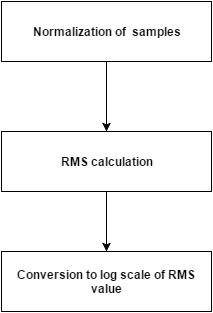
\includegraphics[]{resources/intensity.jpg}
        \caption{Flowchart for intensity calculation}
        \label{fig:figure6}
\end{figure}

\subsubsection{Feature Outputs}
For each song we obtain the following information:
\begin{enumerate}
        \item The Song Name (String) obtained from the filename.
        \item The Intensity (Double)
        \item The MFCC (List of 40 Doubles) 
        \item The Rhythm (List of 32 Doubles)
\end{enumerate}
\par An example set of data is given below (some values removed for clarity):\\
{
        \hspace{20cm} "songName":"Pop-22.mp3",\\
        \hspace{20cm} "intensity":\\
        \hspace{20cm} 58.510281774287414,\\
        \hspace{20cm}"mfcc":\\
        \hspace{20cm}[ 20.7403817933,-.1448360237883,-.10059620606765,....,0.619933641865,2.75522298062],\\
        \hspace{20cm}"rhythm":\\
        \hspace{20cm}[0.0,2.0,6.0,9.0,4.0,14.0,11.0,4.0,2.0,0,12.0,17.0,4.0,9.0,6.0,4.0,0.0]\\
}
Intensity is usually in the 50 - 80  range, MFCC values are around 1.0 except the first value, while rhythm normally lies in the 0.0 to 20.0 region.

\subsection{K-means Clustering}

\subsubsection{Overview}
As mentioned before, at this point in the project, we have completed implementing the K-means algorithm.
We decided to implement it ourselves for two reasons: 
\begin{enumerate}[a.)]
        \item It is a pretty straightforward and simple algorithm.
        \item We wanted to have full control over all aspects related to the implementation: the initialization method, distance metric, etc.
\end{enumerate}
The implementation however is basic in the sense that no modification has been done on the algorithm to better suit the problem domain.\\ 
Some finer points of the implementation are discussed below after quickly going over the algorithm itself. 

\subsubsection{Algorithm}
Let X = { $x_1, x_2,.... ,x_n$ be the set of data points and V = { $v_1,v_2 , ...,v_c$ } be the set of centers. 
        \begin{enumerate}[1.)]
                \item Randomly select 'c' cluster centers. 
                \item Calculate the distance between each data point and cluster centers. 
                \item Assign the data point to the cluster center whose distance from the cluster center is minimum of all the cluster centers. 
                \item Recalculate the new cluster center: 
                        \begin{equation}
                                v_i=\frac{1}{c_i}\sum_{j=1}^{c_i}{x_i}
                        \end{equation}
                \item  Recalculate the distance between each data point and new obtained cluster centers. 
                \item If no data point was reassigned then stop, otherwise repeat from step 3).
        \end{enumerate}

        \subsubsection{Initialization method}
        Commonly used initialization methods are Forgy and Random Partition. The Forgy method randomly chooses k observations from the data set and uses
        these as the initial means. The Random Partition method first randomly assigns a cluster to each observation and then proceeds to the update step, thus
        computing the initial mean to be the centroid of the cluster’s randomly assigned points. The Forgy method tends to spread the initial means out, while
        Random Partition places all of them close to the center of the data set. According to [6], the Random Partition method is generally preferable for
        algorithms such as the k-harmonic means and fuzzy k-means. For expectation maximization and standard k-means algorithms, the Forgy method of initialization is preferable. 
        \par And with these facts in mind, we went for the random initialization method. This method has been used in [2] too although they have also added
        the constraint that the centroids be separated by at least a threshold KL-divergence distance. As the choice of initial centroids have a drastic
        effect on the cluster formed, we have also considered other methods of initialization such as the breakup method which uses the actual data points
        and the scrambled midpoints method which uses synthetic data points as suggested in [4]. However, these techniques are to be implemented in the next phase.

        \subsubsection{Distance Metric}
        Apart from the initialization method, K-means is also highly sensitive to the distance metric used. 
        K-Means is implicitly based on pairwise Euclidean distances between points, because the sum of squared deviations from centroid (that it tries to minimize) is equal
        to the sum of pairwise squared Euclidean distances divided by the number of points [5]. 
        \par    As such, we decided to use Euclidean distance with weights for the three different features added to give us a way to control the metric. Thus, the
        distance between two songs S1 and S2 is given by: 
        \begin{equation}
                Distance(d)=\sqrt[2]{w_I(I_1-I_2)^2+w_M\sum_{i}{(M_{1i}-M_{2i})^2}+w_R\sum_{i}{(R_{1j}-R_{2j})^2}}
        \end{equation}
        Where: $w_I$ , $w_M$  and $w_R$ are the weights for Intensity, MFCC and Rhythm respectively. 

        \subsubsection{Reading the Data Points}
        The feature extractor stores the data as JSON which we read into the classifier using Gson – a Java serialization library that can convert
        Java objects into JSON and back. 
        \par  The choice of JSON was based on the fact that it's easily human readable and there are lots of libraries in a variety of languages
        to read it if needed. 
        \begin{figure}[h]
                \centering 
                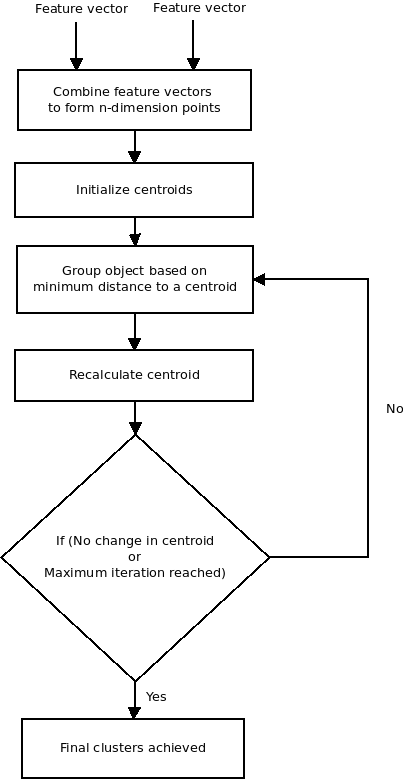
\includegraphics[scale=0.55]{resources/kmeans.png}
                \caption{K-means clustering}
                \label{fig:figure7}
        \end{figure}


